\section{Cloud Grading Architecture With OpenEdX}
\label{sec:arch}

We adopt a narrow Unix-like view of an autograder: it is a
stateless command-line program that, given a student work submission and
a rubric, computes a score and some textual feedback.  We then treat
separately the question of how to connect this program to an LMS.

All other policy issues---whether students can resubmit homeworks, how
late penalties are computes, where the gradebook is stored, any other
LMS behaviors---are out of scope, as is the question of whether these
autograders should replace or supplement manual grading by instructors.

\subsection{Student Experience}

Our initial implementation of \texttt{rag} was designed to work with
Coursera, but both the interface and student experience are similar
between Coursera and OpenEdX.  A logged-in learner navigates to a page
containing instructions and handouts for a homework assignment;
when ready, the learner submits a single file or a
\texttt{tar} or \texttt{zip} archive through a standard HTTP
file-upload form.  A short time later, typically less than a minute, the
learner can refresh the page to see feedback on her work from the
autograder.  Depending on the course policy, she may be able to improve
her work and resubmit.

\subsection{Interface Between Autograders and OpenEdX}

\tbd{point to OpenEdX documentation}

OpenEdX defines a 
protocol~\uf{edx-partner-course-staff.readthedocs.org/en/latest/exercises\_tools/external\_graders.html}
for interacting with so-called ``external
graders.''  When an OpenEdX student submits an assignment that is
to be graded by an external grader, the student's submitted file goes
into a persistent named queue called an XQueue; each course has its own
XQueue.  OpenEdX exposes a 
authenticated RESTful API \tbd{need citation for RESTful API} through which an
external grader can retrieve a student assignment from an XQueue and
later post back a numerical grade and textual feedback.  
The student submission form can be configured to include additional
metadata for the autograder; we use that field to distinguish different
assignments so that the autograder knows which rubric files must be used.

Retrieving an
assignment and posting back a 
grade are separate queue operations, to allow for autograders that may
take a long time to run.  
If the autograder polls the XQueue and finds it empty, the grader
process sleeps for awhile and tries again.  (In the future we will allow
idle autograders to kill themselves.)
If an assignment is retrieved but no grade is posted back before a
preset timeout, OpenEdX returns the assignment to the queue, where it will
eventually be picked up again by another autograder instance.
Therefore, if an autograder crashes while grading an assignment, no
student work is lost.

This architecture makes it relatively straightforward to absorb a large
burst of assignment submissions: since  the autograders 
  themselves are stateless and the only state is in the XQueues,
we simply deploy additional copies of
the VM instances on Amazon's cloud.  Since grading is embarrassingly
task-parallel, each autograder instance we deploy results in a linear
increase in the rate at which the queue is serviced.  
Even our most sophisticated autograders take less than one
machine-minute per assignment, so at less than 10 cents per machine-hour,
MOOC-scale 
autograding is cost-effective and fast: even with
thousands of assignments being submitted in a 50,000-learner course,
students rarely waited more than a few minutes to get feedback.

OpenEdX also supports an alternative protocol in which each student
submission event triggers a call to a RESTful autograder endpoint,
effectively having OpenEdX ``push'' submissions to the autograder rather
than having the autograder ``pull'' them.  We do not use this
alternative protocol because it would thwart this simple scaling trick
and because we might find ourselves unable to limit the rate at which
submissions were pushed to our autograders.

The external grader does not have access to
the identity of the learner; instead, an obfuscated token identifies the
learner, with the mappings to the learners' true identities maintained only on the
OpenEdX LMS.  Hence no sensitive information connecting a work product
to a specific student is leaked if the autograder is compromised.

\begin{figure}
  \centering
  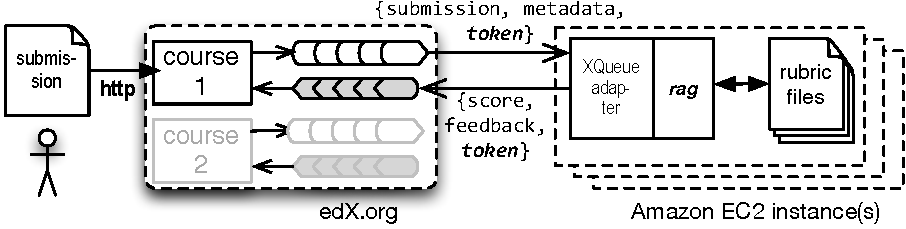
\includegraphics[width=0.75\textwidth]{figs/autograder_arch.pdf}
  \caption{\label{fig:arch}
  Since our autograders rely on many libraries,
  tools, support files, and so on, we encapsulate the autograder in a
  virtual machine image that is deployed on Amazon Elastic Compute Cloud.
  When a new instance is started, the autograder script automatically runs from
  \texttt{/etc/init.d} and examines a deploy-time environment variable
  to get obtain the credentials needed to make calls to the XQueues.}
\end{figure}


\subsection{Rubric Files}

autograder, rubric file

current refactoring to allow rubric files to be pulled on demand and
updated in place

\subsection{CI Workflow for Autograders}

For continuous integration, we use Travis-CI, which is integrated with GitHub and runs on submission of patches for acceptance ("pull request" in GitHub terminology), as well as other events. Users develop on their own forks of a repository, then submit pull requests back to the main repository when finished. Even when not finished, pull requests to the main repo may draw attention that can keep the team informed or resolve issues.

When Travis is triggered, it typically loads a new virtual host, installs runtime binaries and basic libraries, clones the associated GitHub repo including .travis.yml, installs dependencies, and runs indicated tests.
Some .travis.yml files are very simple, using mostly defaults. This one only has specific differences of using an old Ruby version before Travis calls the commands under the 'script:' key, which start the test suites. Those commands use 'bundle exec' to choose rspec and cucumber versions indicated in the project's Gemfile. The tests are in the repo's spec and features folders, and their output is included in the record of the build run.

\begin{figure}[!htbp]
  \begin{minipage}{0.70\textwidth}%
  \lstset{tabsize=1,basicstyle=\scriptsize\ttfamily}
  \lstinputlisting{figs/travis.yml}%
  \end{minipage}
  \caption{\label{fig:rag-ci}%
  Typical .travis.yml file.
}
\end{figure}

For the autograders themselves, it runs the rspec and cucumber tests located in the default spec and features directories. For the separate homework repositories that use the autograders as a library, we used cucumber Scenario Outline AST tables to organize tabular input and assert results. Our cucumber tests then execute them via the Open3 library in order to control output streams and return codes. In the homework repos, we also added a cucumber feature to script the install and verify the configuration of the autograders, which simplified the use of multiple repositories, especially for new users.

\begin{figure}[!htbp]
  \begin{minipage}{0.99\textwidth}%
  \lstset{tabsize=1,basicstyle=\scriptsize\ttfamily}
  \lstinputlisting{figs/ci_feature.txt}%
  \end{minipage}
  \caption{\label{fig:rag-ci}%
  Cucumber feature Scenario Outline AST table for CI.
}
\end{figure}


\subsection{Robustness and Security}

Since ill-behaved student code is a concern, there are various layers of
security.  For the RSpecGrader, the tests must be run in the same
process as the student's code.  They are run in a separate interpreter
thread that is protected by a timeout and in which large 

Multiple layers of security: watchdog timers, sandboxed interpreter, threads. Hollingsworth 1960 observed that it was possible for students to submit programs that deliberately damage the autograder.

Trustworthiness: because we control the VM image in which the
  autograder runs and the grades are recorded to a central queue server
  which we also control, students cannot tamper with the autograder's
  results or functioning.

Sandboxing: while our RSpec-based autograder performs much of its
  own sandboxing, even if student code escapes the sandbox we can shut
  down and undeploy the VM.  

  TBD Watchdog timers that do this if miss several heartbeats.




